\section{Results}
\par The experiment was carried out across the first half of the Spring 2017 quarter at Cal Poly. 130 students signed up across 4 classes. By the end of the experiment, just over 3200 answers had been submitted to the application.

\par Currently, we only have access to exam data from Introduction to Operating Systems. The exams were held completely through an online quiz form, making it easy to analyze the resulting data. Data collection for the rest of the classes is ongoing.

\subsection{Limitations}
\par Certain restrictions were necessary in order to run this experiment. Most importantly, according to Cal Poly's human research regulations, studies about educational tools must be offered to all participants in a class. Thus, there was no true "control group" since any student could opt-in or opt-out of using the application.

\subsection{Overall Data}
\par First, consider the relationship between a student's overall score on the midterm and their Commitment (\textbf{\hyperref[fig:comm_vs_score]{Figure \ref*{fig:comm_vs_score}}}). No student that actively used the app (more than 10 Commitment) got less than 30/50 as a final score. This supports the idea that students benefit from consistent repetition over a longer period of time.
 
 \begin{figure}[h]
 	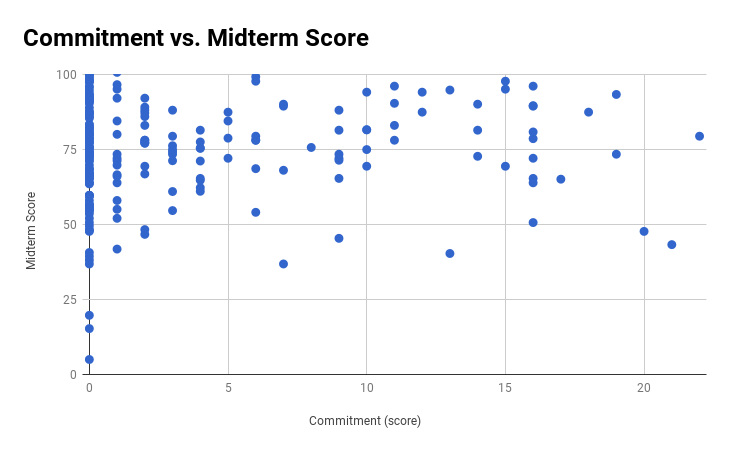
\includegraphics{figures/commitment-data1}
 	\caption{Graph of Commitment versus the student's score on the midterm.}
 	\label{fig:comm_vs_score}
 \end{figure}
 
 \par Next, consider the mean of all midterm scores between students that didn't answer \textit{any} questions vs. the ones that did. Students that didn't answer any questions in the app scored slightly higher on average than the students that didn't.
  
 \begin{tabular}{ r c c }
  & Users & Non-users \\
  \hline			
 Midterm Average & 39.37 & 36.27 \\
 Population Size & 43 & 21
\end{tabular}

\subsection{Individual Questions}
Certain questions on the midterm matched closely with the content of the questions that were repeated on Polycommit. We can match scores 

% TO DO: Put statistics for individual questions here. Note that deadlock wasn't improved by much, SJF actually got worse. Bring up possibility that students who sought out the app perhaps had less prior understanding of the course content or less consistent original study habits, leading to a selection bias that made them perform more poorly.

% Then, bring in statistics from the final survey where respondents said that they enjoyed using the app, and thought it improved their scores on quizzes and exams.
 